\begin{minipage}[t]{100mm}
\vspace{3mm}
\section*{Ikke-kommutativ studenterrådgivning}
\emph{Kære brevkasse}

\emph{Hvordan finder jeg ud af om jeg er en hun\-dværg eller en han\-dværg?}

\emph{Hilsen, en forvirret dværg}

\subsection*{Svar}
Kære forvirret dværg

Det er ikke særligt svært at finde ud af, om du er en hundværg eller en handværg, da forskellen kan bestemmes ved at bemærke nogle grundlæggende biologiske egenskaber. Det er alment kendt at hundværge foretrækker at slibe deres stridsøkser med kvartssand

{\flushright\emph{Hilsen den ikke-kommutative studenterrådgivning}}

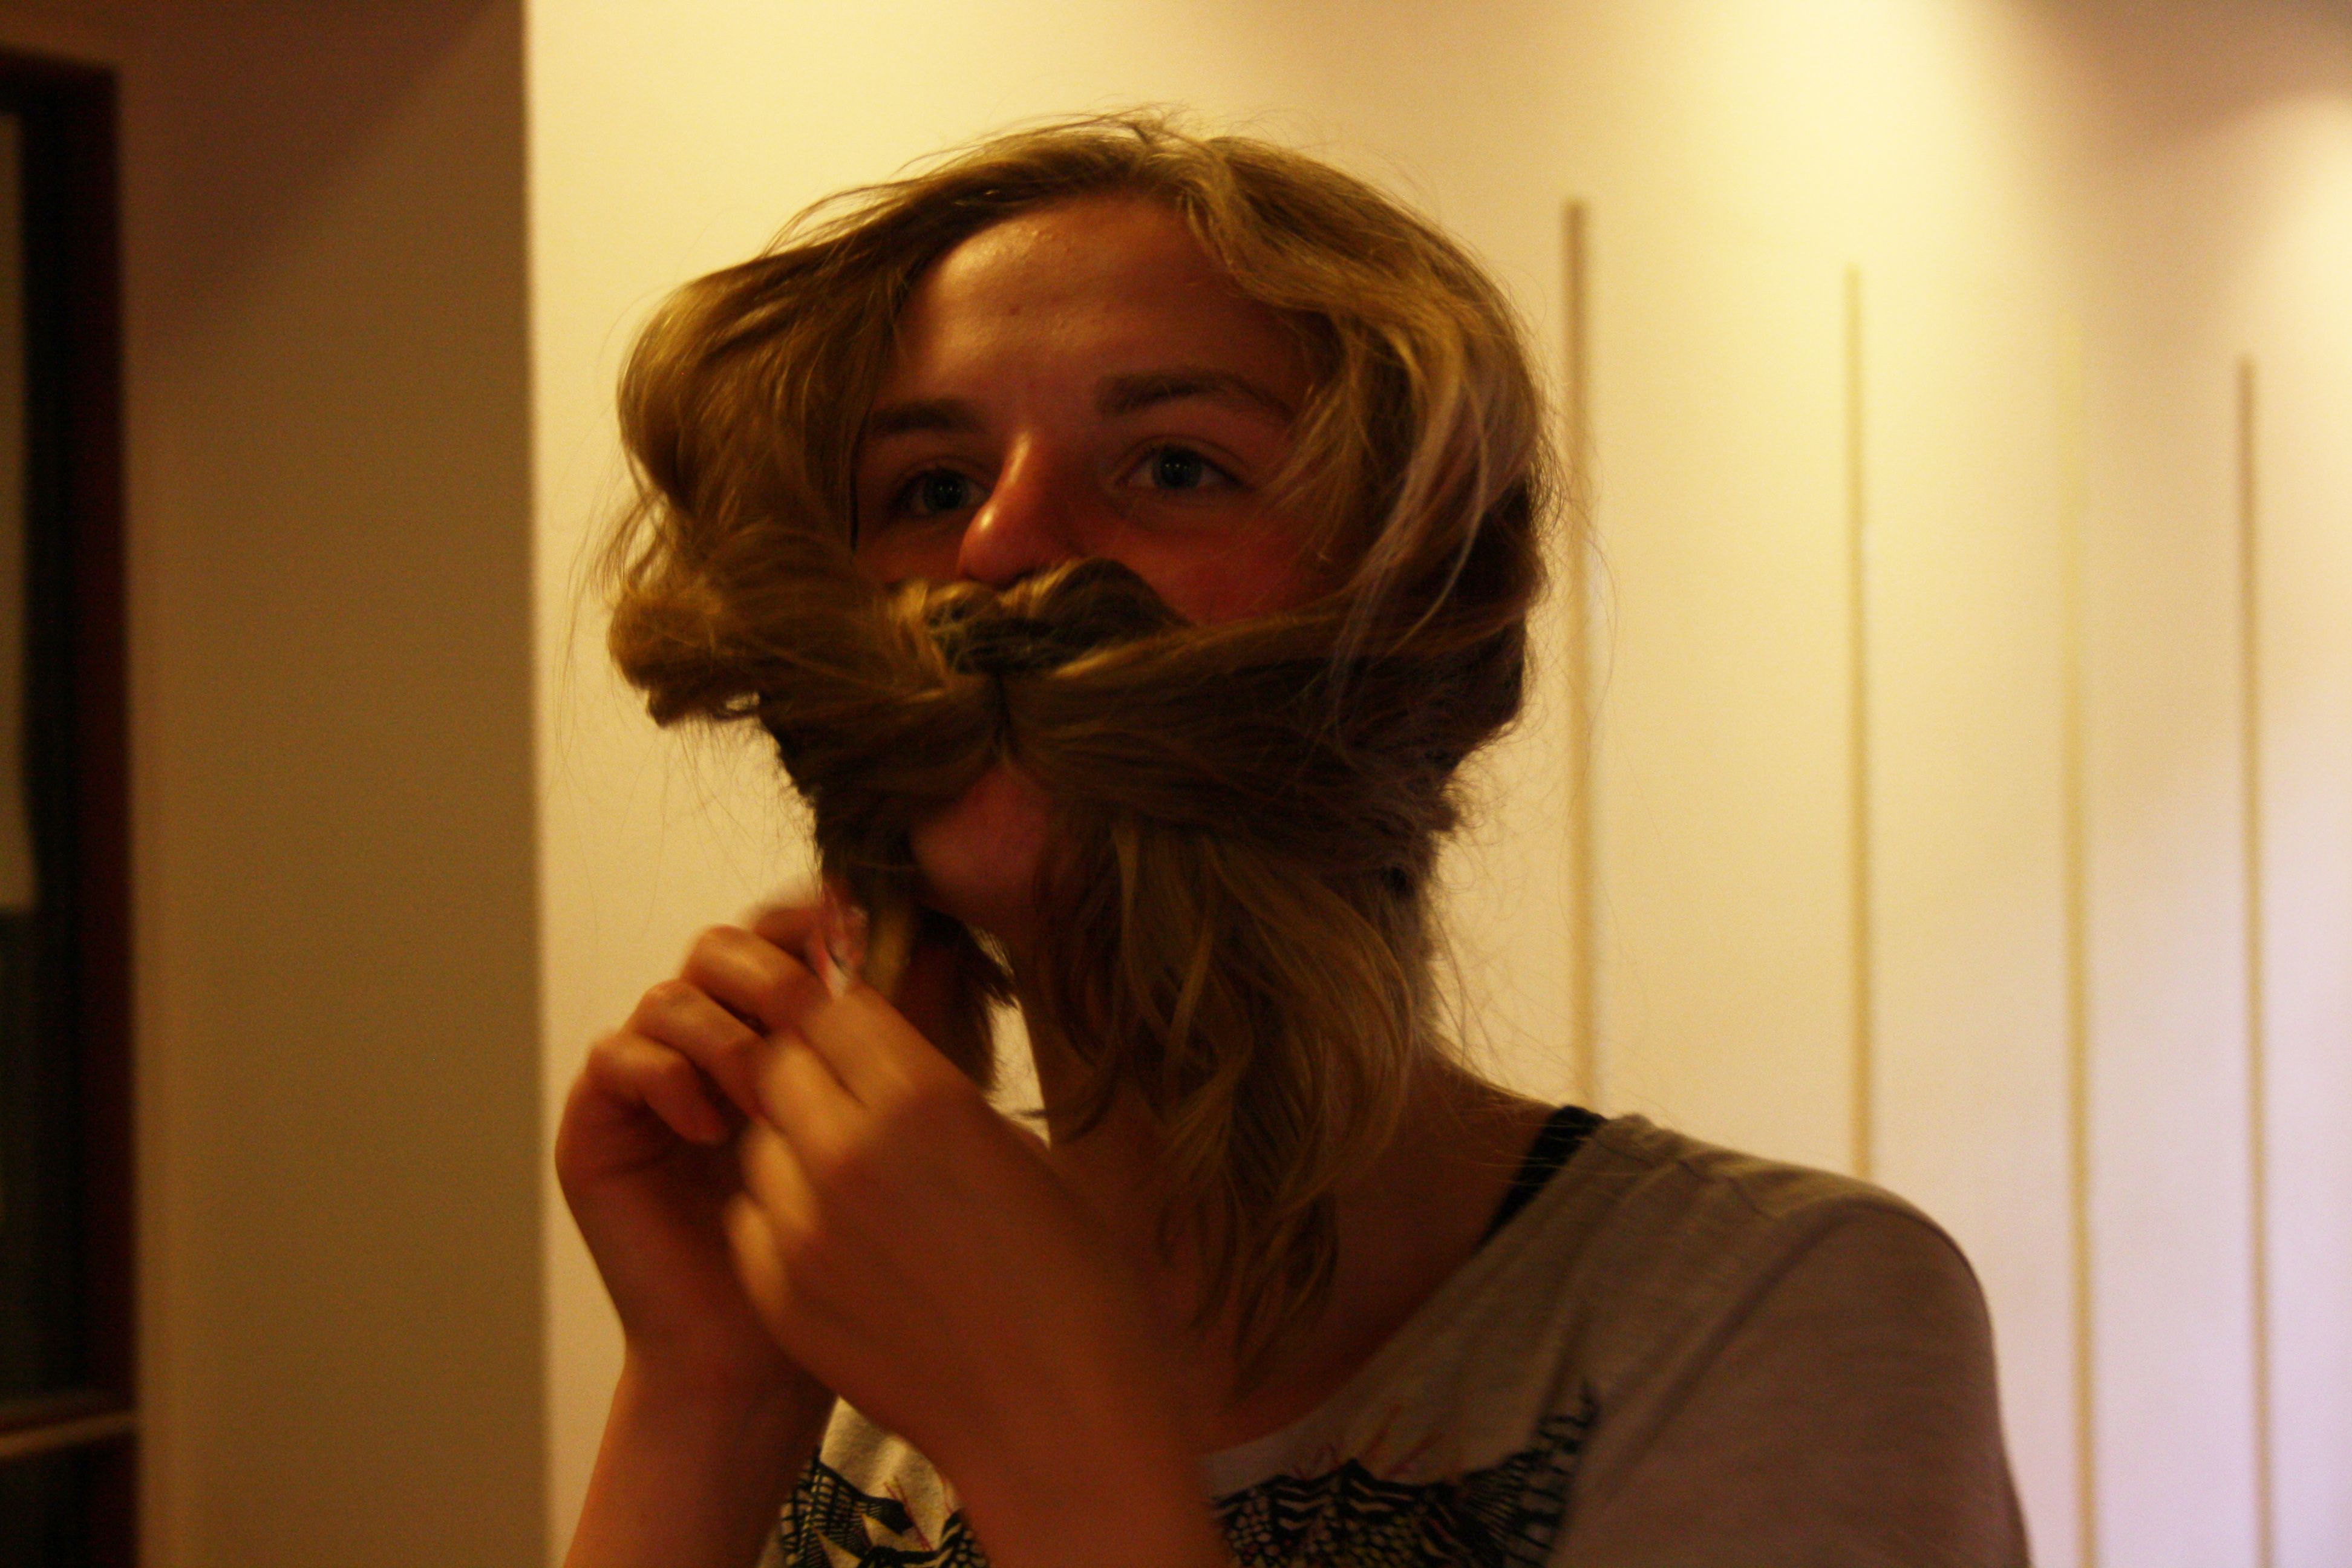
\includegraphics[width=100mm]{kum.jpg}


\end{minipage}

